\chapter{Storage System Control} \label{chapWhControl}

This chapter deals with the control of the operations of a storage system. Controlling the performance of a storage system is a crucial activity to maximise its productivity.

\section{Performance assessment (P8)}
This paragraph illustrates the approaches to evaluate the performance of a storage system. The measurement of the performance of a storage system involves a wide number of metrics since storage systems exist at any stage of the supply chain ~\cite{Accorsi2017a_wh, Malmborg2000, Manzini2007, Staudt2015}.

\subsection{Model-driven methods (D4)}

A storage system works as an intermediate buffer of a supply chain. It receives material flows from suppliers, and generate material flows directed to the customers. Many information flows connect suppliers and customers with the operations of a warehouse. Mapping this flow is a common technique to assess the exchange of materials and information from a qualitative point of view. The Business Process Model and Notation is used to identify entities, flows and responsibilities. When applying the BPMN to a storage system:

\begin{itemize}
    \item Activities are tasks necessary for the storage and handling of SKUs;
    \item The events identify when an activity is terminated (e.g. a put-away or a picking list);
    \item Gateways describe a different variant of the process (e.g. value-added activities as packing, quality control, labelling).
    \item Pools identify the operators and the offices of the storage system, identifying their responsibilities.

\end{itemize}

BPMN defines a qualitative map of the production processes useful for manager and practitioners to identify the way their processes are realised. More difficult is the assessment of these processes from a quantitative point of view. For this reason, a dashboard of KPIs is introduced, coherently with the ontology of \ref{secOntology_wh}. The KPIs used in these chapters refers to the problems defined in \ref{secDecisionPatterns}. KPIs are organised according to four classes ~\cite{Tufano2018_wh}:

\begin{enumerate}
    \item Logistic KPIs, evaluate the logistic impact of a certain solution. They use metrics like time, distance and the performance parameters introduced in Paragraph \ref{secOntology_wh}.
	\item Cost KPIs, evaluate the economic sustainability of a given solution. They are expressed in \euro{} or other currency.
	\item Energy KPIs, evaluate the energy needed to feed a given solution. They use metrics as kW and kW/h.
	\item Environmental KPIs, evaluate the environmental impact of a given solution. They are expressing the equivalent $CO_2$ produced per year.

\end{enumerate}

Table \ref{tab_kpis} identifies which KPI is relevant to each problem. In general, each problem can be assessed from multiple perspectives.

% INSERT tab_kpis
\begin{figure}[hbt!]
\centering
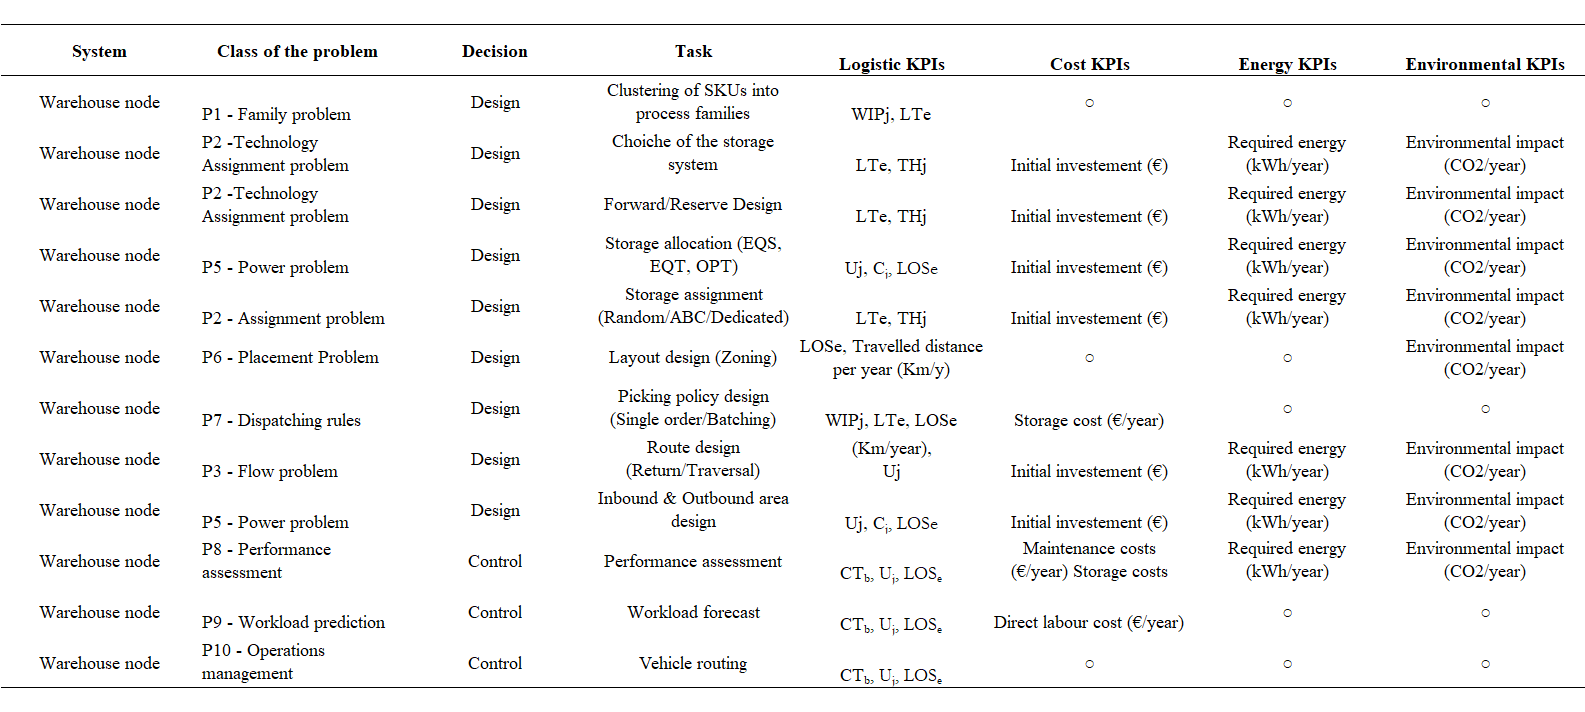
\includegraphics[width=0.9\textwidth]{SectionWarehouses/control_figures/tab_kpis.png}
\captionsetup{type=table}
\caption{KPIs to evaluate the solutions to problems in a distribution network.}
\label{tab_kpis}
\end{figure}

\subsection{Data-driven methods (D2, D4)} \label{secDataDrivenAnalysisWh}

While the operations of different storage systems have similar patterns, their data can have different organisation and features. The assessment of the performance of a storage system depends on the type and quality of the data recorded. Figure \ref{fig_diagnosis_wh_DataDriven} illustrates the data pipelines connecting the attributes of the dataset, the analysis and the performance metrics identified by Table \ref{tab_kpis}.

% INSERT fig_diagnosis_wh_DataDriven
\begin{landscape}
\thispagestyle{empty}
\begin{figure}[hbt!]
\centering
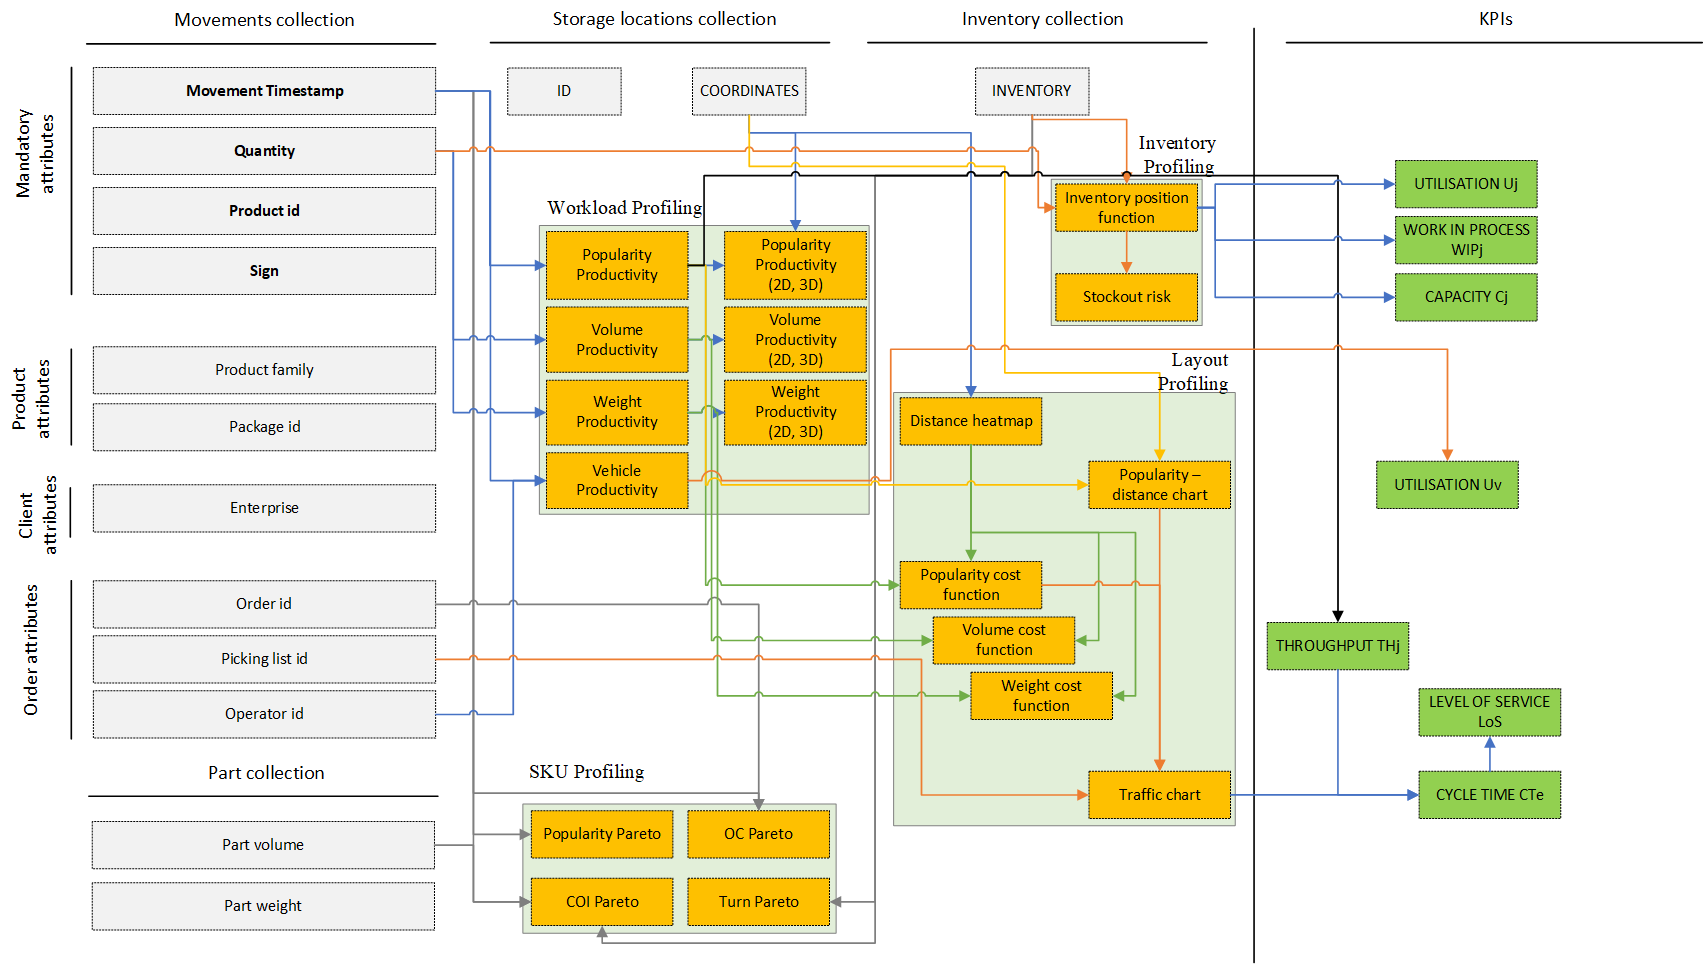
\includegraphics[width=1.5\textwidth]{SectionWarehouses/control_figures/fig_diagnosis_wh_DataDriven.png}
\captionsetup{type=figure}
\caption{Connections between attributes, analyses and KPIs}
\label{fig_diagnosis_wh_DataDriven}
\end{figure}
\end{landscape}

The analysis (identified by the orange blocks in Figure \ref{fig_diagnosis_wh_DataDriven}) are grouped into four main areas, depending on the entity of the warehouse they affect: the SKUs, the inventory level, the workload, and the layout.

\subsubsection{SKU profiling}
Warehouses contain thousands of different SKUs. For this reason, it is necessary to profile them and approach the design and control of the operations differently depending on the SKUs profile. \par

We introduce four different profiling indexes; some indexes are defined differently for inbound and outbound operations.

\begin{itemize}
    \item The popularity index $Pop_i^+$, $Pop_i^-$ counting the number of put-away/picks of SKU $i$;
    \item The turn index $Turn_i=\frac{Qty_i^-}{\bar{I_i\left(t\right)}\ }$; where $Qty_i^-$ is the outbound quantity of SKU $i$ measured in parts or $dm^3$, and $\bar{I_i\left(t\right)}$ is the mean value of the inventory function of part $i$ measured in parts or $dm^3$. The turn measures the rotation of the inventory of a part.
    \item 	The cube-per-order index $COI_i^+=\frac{Pop_i^+}{\bar{I_i\left(t\right)}\ }$, $COI_i^-=\frac{Pop_i^-}{\bar{I_i\left(t\right)}\ }$; where $Pop_i^+$, and $Pop_i^-$ are the inbound or outbound popularity and $\bar{I_i\left(t\right)}$ is the mean value of the inventory function of part $i$ measured in $dm^3$. The COI mixes the two metrics above to have both a measure of the number of accesses and the space occupied by a part ~\cite{Haskett1963, Malmborg1990}.
    \item 	The order completion index $OC_i\ =\sum_{e:i\in e}\frac{1}{card(e)}\ $; where $e$ is an order or a  picking list. The index measures the relative importance of a part $i$ to complete a single order.
\end{itemize}

Mapping all these indexes provide a behaviour of each single SKU. This indexes can be grouped using the Pareto curve, and the frequency analysis to investigate the behaviour of an entire storage system (see Figure \ref{fig_wh_profile}).\footnote{The source code of Figure \ref{fig_wh_profile} is available \href{https://github.com/aletuf93/logproj/blob/master/examples/WH_02\%20Warehouse\%20indexes\%20assessment.ipynb}{here}.
}

% INSERT fig_wh_profile
\begin{figure}[hbt!]
\centering
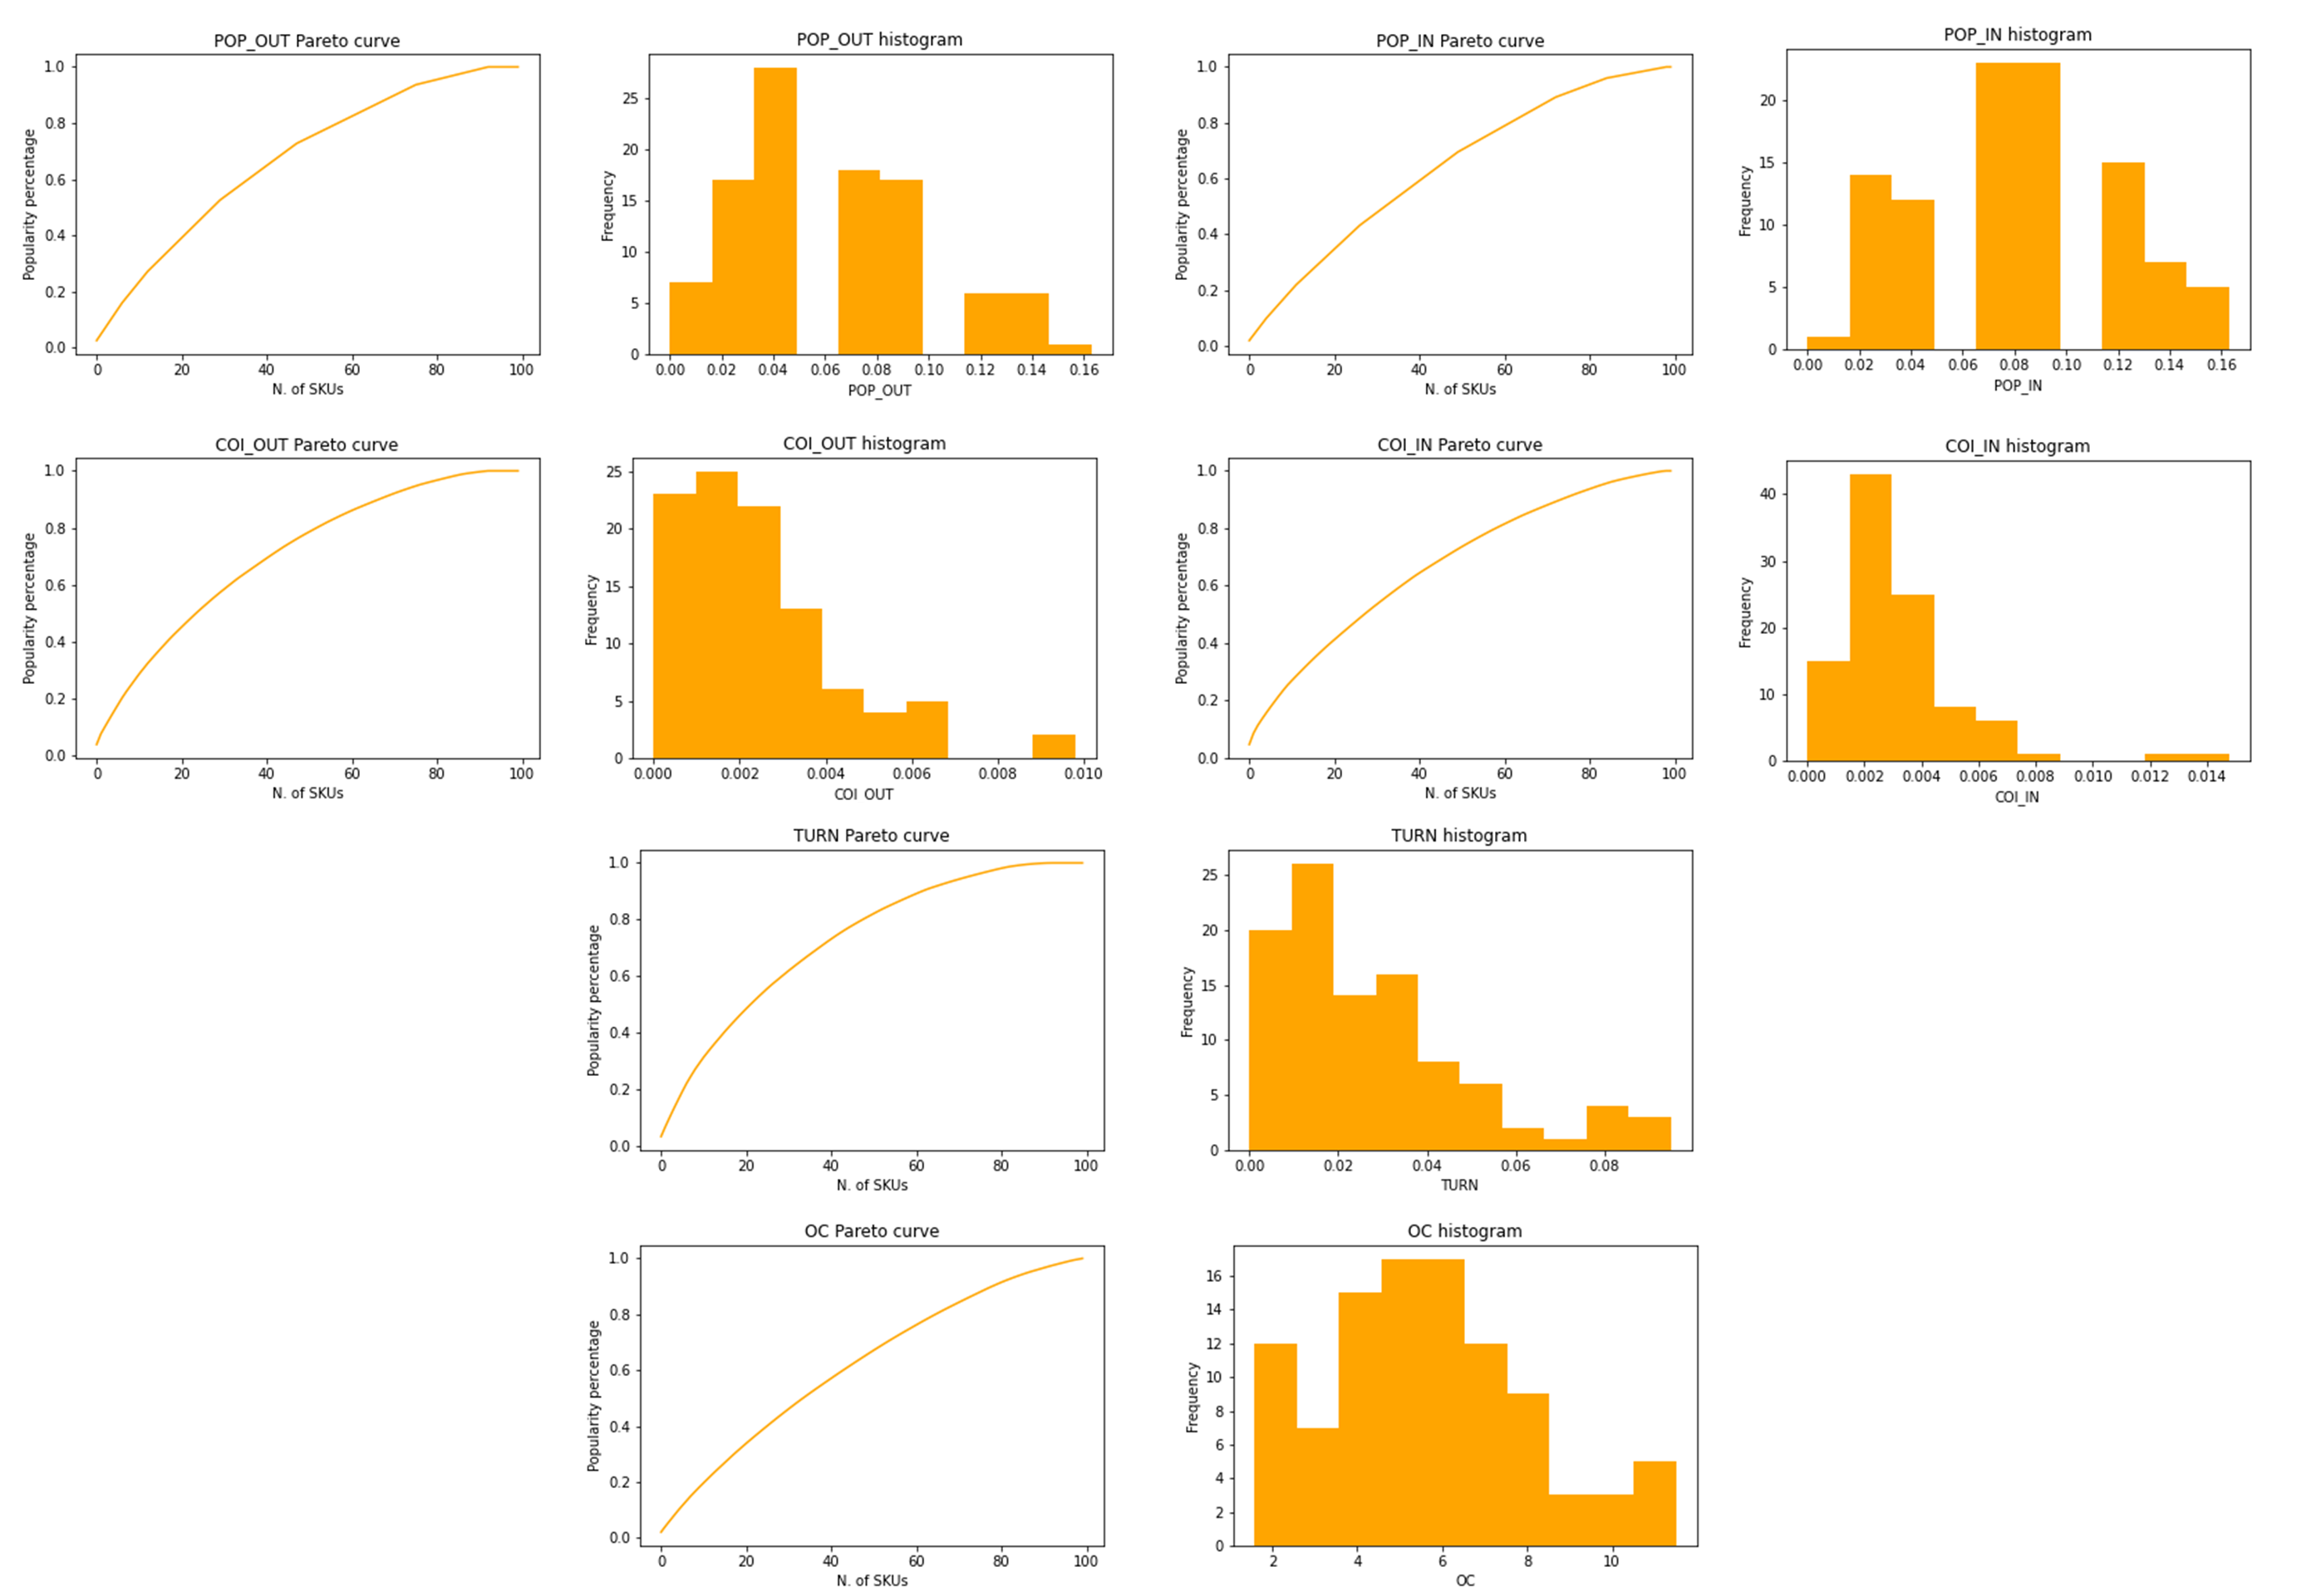
\includegraphics[width=1.0\textwidth]{SectionWarehouses/control_figures/fig_wh_profile.png}
\captionsetup{type=figure}
\caption{Pareto curves and frequency analysis of the indexes to classify the SKUs of a storage system.}
\label{fig_wh_profile}
\end{figure}

\clearpage

\subsubsection{Inventory profiling}
Inventory profiling is a fundamental activity to assess the efficiency of a storage system. The space efficiency of a storage system depends on the degree of saturation. The less the available space, the better the utilisation of the storage system. Nevertheless, the higher the saturation of the storage system, the higher the probability to have a lack of space for incoming goods. The design of the inventory level is analysed in paragraph \ref{secInventoryDesign} and relies on the results of the inventory profile defined here.\par

The definition of the inventory function $I_i(t)$ for each SKU $i$ is a preliminary activity to profile the inventory of a storage system. When the dataset contains an inventory snapshot $I_i(\tau)$ at time instant $\tau$, the inventory is obtained by considering:

\begin{equation}
    I_i\left(\tau+\epsilon\right)=I_i\left(\tau\right)+M_i^+\left(\tau+\epsilon\right)-M_i^-(\tau+\epsilon)
    \label{eq_wh_inventory1}
\end{equation}

\begin{equation}
    I_i\left(\tau-\epsilon\right)=I_i\left(\tau\right)-M_i^+\left(\tau+\epsilon\right)+M_i^-(\tau+\epsilon)
    \label{eq_wh_inventory2}
\end{equation}

When there is no inventory snapshot it is possible to use the formulae (\ref{eq_wh_inventory1}), and (\ref{eq_wh_inventory2}) by setting $I_i\left(\tau\right)=0$. The estimate of $I_i\left(t\right)$ is obtained by shifting the function to positive values $I_i\left(\tau\right)=I_i\left(\tau\right)-\min(I_i\left(\tau\right))$ when $\min{\left(I_i\left(\tau\right)\right)}<0$.\par

By summing the inventory functions for all the SKUs, it is possible to measure the saturation of the storage system. It is recommendable to measure $I(t)$ using $dm^3$; otherwise, the estimate of the global inventory function will not be accurate using the number of parts. Figure \ref{fig_inventory_profile} illustrates the inventory function $I(t)$ of a storage system, together with the frequency analysis, and the cumulative distribution functions. The cumulative distribution function is used to design the inventory level of the warehouse (see section \ref{secInventoryDesign}). \footnote{The source code of Figure \ref{fig_inventory_profile} is available \href{https://github.com/aletuf93/logproj/blob/master/examples/WH_03\%20Warehouse\%20Inventory\%20assessment.ipynb}{here}.}


% INSERT fig_inventory_profile
\begin{figure}[hbt!]
\centering
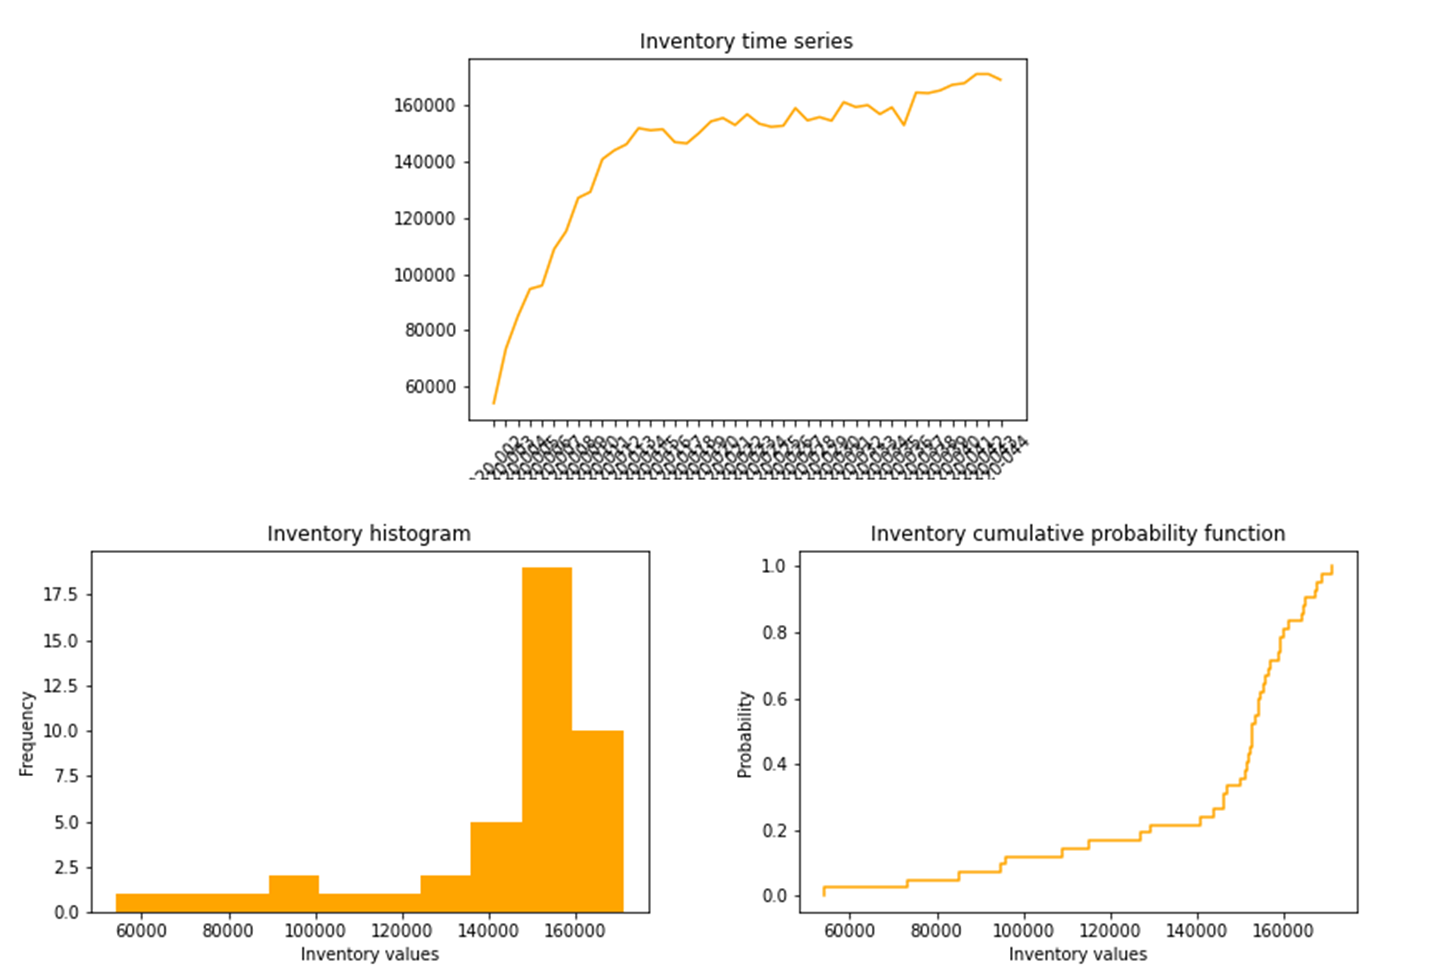
\includegraphics[width=1.0\textwidth]{SectionWarehouses/control_figures/fig_inventory_profile.png}
\captionsetup{type=figure}
\caption{Inventory profile of a storage system.}
\label{fig_inventory_profile}
\end{figure}

\clearpage

\subsubsection{Workload profiling}
Workload profiling aims at assessing patterns of workload per different types of areas or vehicles of the storage system. The workload of a storage system is measurable using:

\begin{itemize}
    \item The popularity $Pop_i^+(t)$, $Pop_i^-(t)$, indicating the number of accesses to part $i$;
	\item The volume $Vol_i^+(t)$, $Vol_i^-(t)$, indicating the put-away or picking volume of part $i$, calculates as quantity times volume of a single part;
	\item The weight $W_i^+(t)$, $W_i^-(t)$, indicating the put-away or picking weight of part $i$, calculated as quantity times weight of a single part.

\end{itemize}

The quantity is rarely used as a workload estimator since the picking, or put-away quantities rarely have an effect on the operations. These functions refer to single parts and can be aggregated at any level, defining the workload of:

\begin{itemize}
    \item the entire storage system;
    \item a specific area of the storage system;
    \item a vehicle or picker.

\end{itemize}

These analyses consider a single independent variable (i.e. the time $t$). By considering the coordinates of the storage locations, it is possible to define multivariate functions to classify the operations of a storage system. Figure \ref{fig_workload_profile2D} illustrates the workload of a storage system using a single dimension (i.e. the time), two dimensions (i.t. the length and the depth of the storage system), and three dimensions (i.e. illustrating the workload within the warehouse space).\footnote{The source code of Figure \ref{fig_workload_profile2D} is available \href{https://github.com/aletuf93/logproj/blob/master/examples/WH_01\%20Warehouse\%20productivity\%20assessment.ipynb}{here}.}


% INSERT fig_workload_profile2D
\begin{figure}[hbt!]
\centering
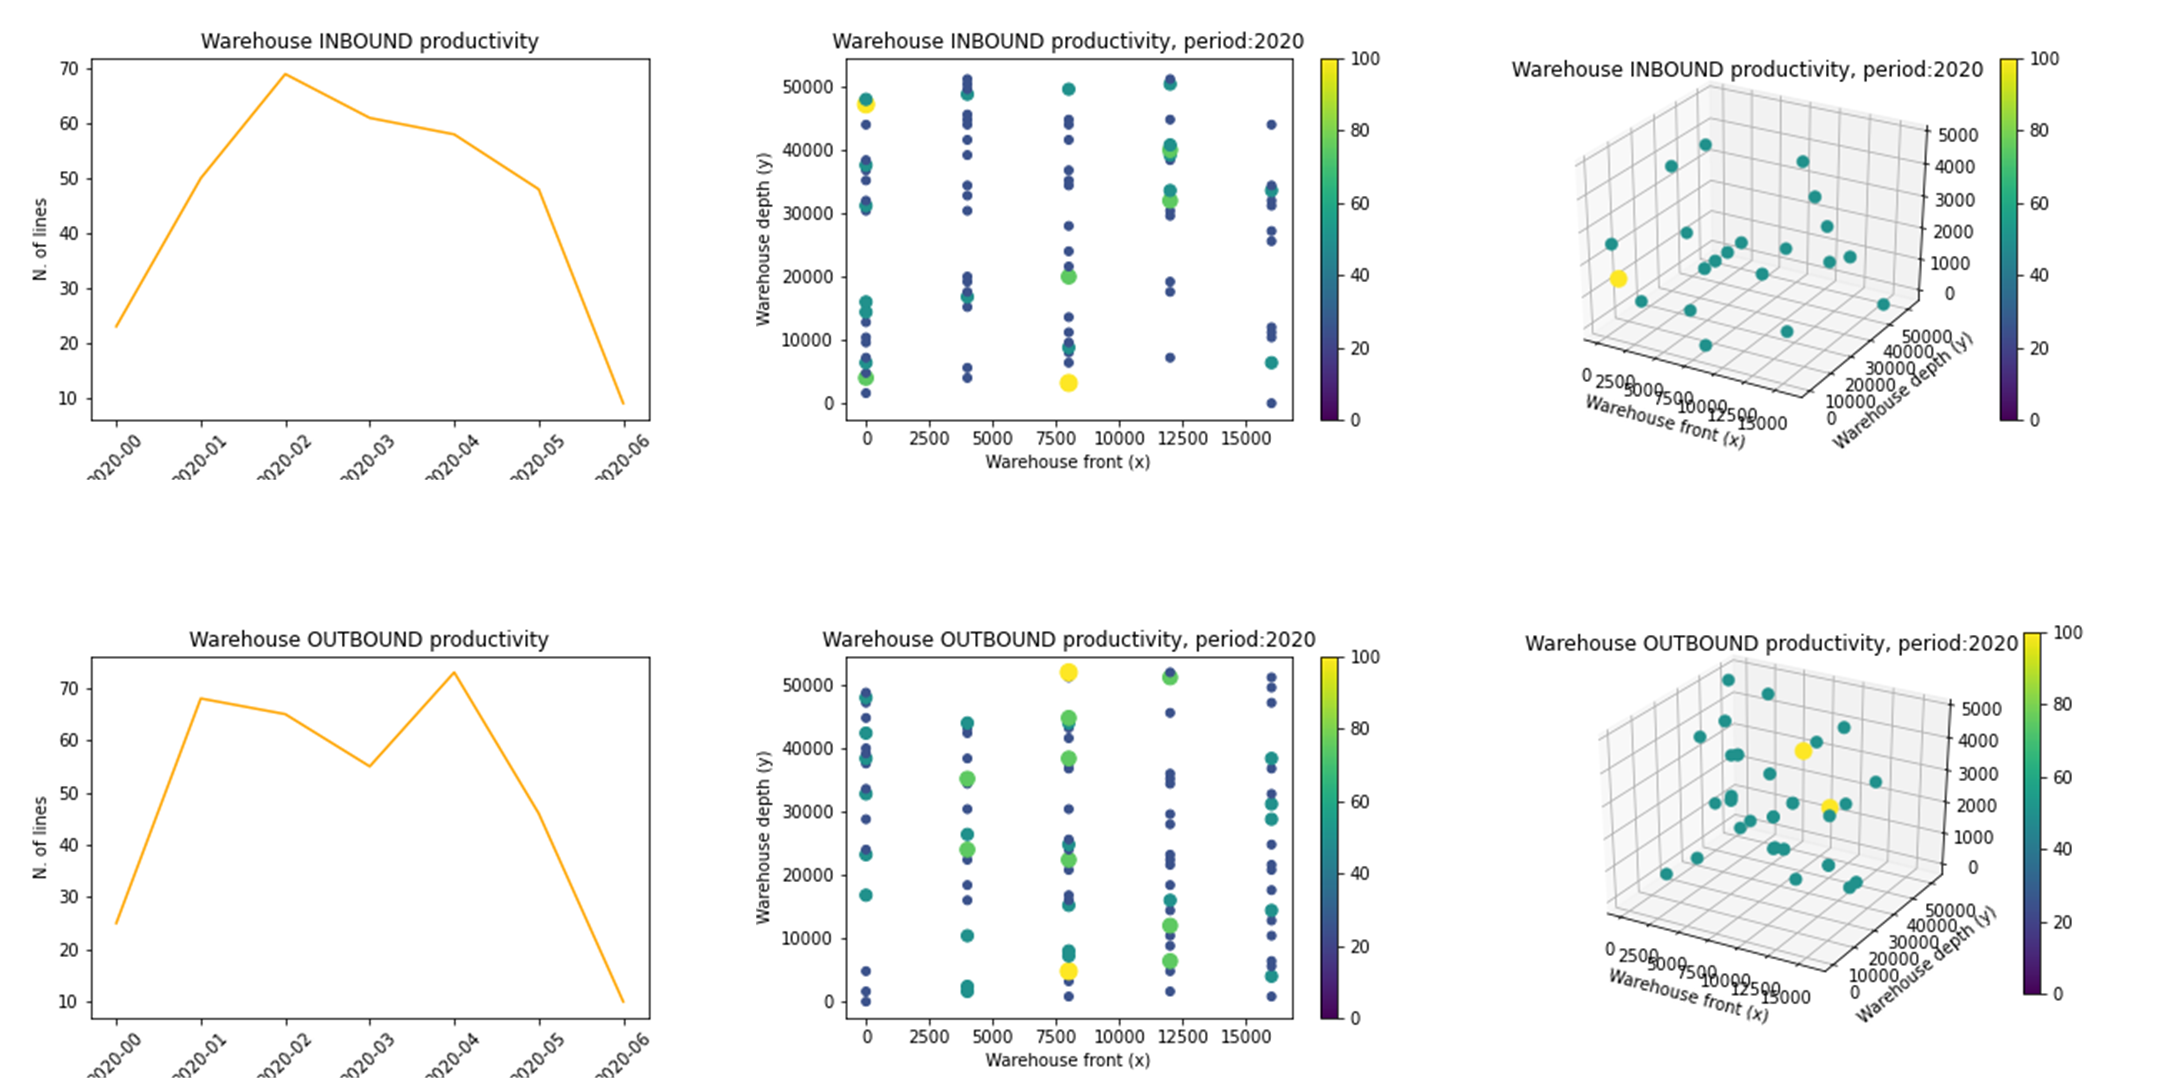
\includegraphics[width=1.0\textwidth]{SectionWarehouses/control_figures/fig_workload_profile2D.png}
\captionsetup{type=figure}
\caption{1-dimensional, 2-dimensional, and 3-dimensional popularity workload analysis.}
\label{fig_workload_profile2D}
\end{figure}

\clearpage

\subsubsection{Layout profiling}
Profiling the behaviour of the resource on the layout of a storage system is the key to identify sources of inefficiencies. By considering the rectangular (also known as “city-block”) distance between the I/O area and each single storage locations, it is possible to identify which locations are closer to reach. Placing the items with a high number of accesses close to the I/O point may increase the efficiency of a storage system.\par

By analysing the distance to reach the storage location where an SKU $i$ is placed, and the popularity of the SKU $i$, it is easy to identify which SKUs are far from their optimal location, and generate a long travelling distance that can be avoided ~\cite{Manzini2018}.\par

Finally, it is important to identify where the traffic is located within a storage system.  When storage location coordinates are known, it is possible to define a graph G(V,E) as introduced in \ref{secNonRelStructWh}. The distance between a storage location and the input and output point is a piece of important information to identify the locations where t place SKUs with the highest popularity indexes (see the chart in the top left panel of Figure \ref{fig_layout_profile}).\footnote{The source code of Figure \ref{fig_layout_profile} is available \href{https://github.com/aletuf93/logproj/blob/master/examples/WH_04\%20Warehouse\%20layout\%20assessment.ipynb}{here}.} \par

By solving the shortest path between the sequence of locations visited by a picking list, it is possible to identify the traffic within the aisles of the storage system. This procedure reveals the travelled distance for each picking list and the part of the aisles where each vehicle travelled. A traffic chart is used to reveal this information (see the chart in the top right panel of Figure \ref{fig_layout_profile}). \par

The optimisation of a storage system can be obtained by placing the SKUs in a different storage location, to reduce the travelled distance to pick them. The degree of suboptimisation of a storage system is measurable by using a chart plotting the popularity, and the distance from the input and output points for each storage location ~\cite{Manzini2018}. The storage system is optimised when the chart is similar to a negative exponential function (see the chart in the bottom right panel of Figure \ref{fig_layout_profile}). Otherwise, the storage system is sub-optimised (see the chart in the bottom left panel of Figure \ref{fig_layout_profile}). \par

% INSERT fig_layout_profile
\begin{figure}[hbt!]
\centering
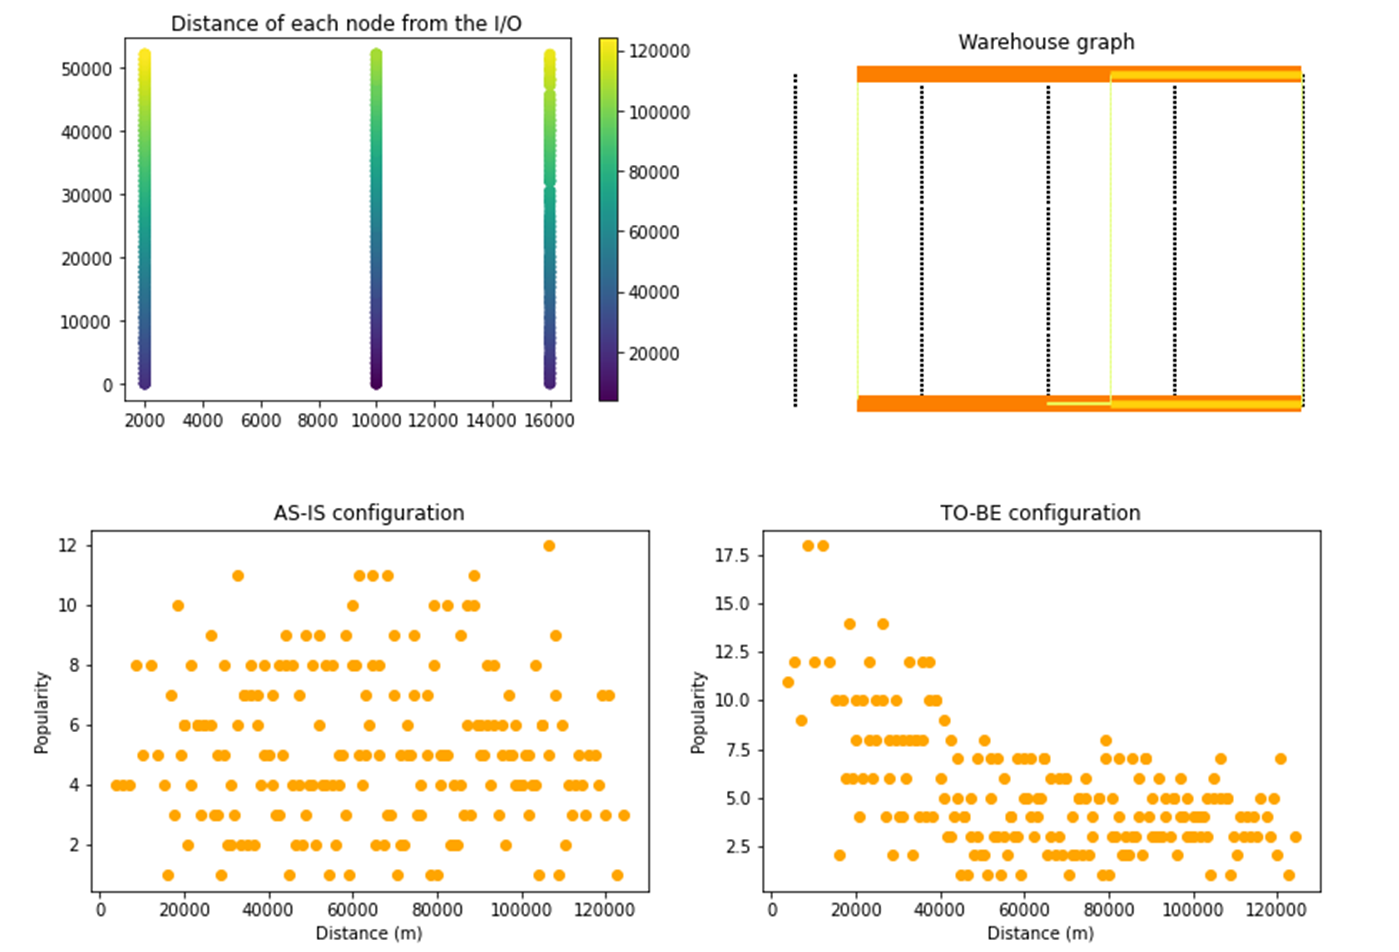
\includegraphics[width=1.0\textwidth]{SectionWarehouses/control_figures/fig_layout_profile.png}
\captionsetup{type=figure}
\caption{Analyses to profile the layout of a storage system.}
\label{fig_layout_profile}
\end{figure}

\clearpage

\section{Workload prediction (P9)}
Storage system datasets track both the behaviour of its supplier and customers by considering put-away (labelled with the “+” sign), and pickings (labelled with the “-“ sign). For this reason, they have all the data to make forecasts of the workload in the future.

\subsection{Model-driven methods (PD2)}
Classic time series methods help to model and predict the workload of the storage system in the future. Usually, the number of movements (i.e. the lines) is much more representative than the quantities (more used in production forecasts) ~\cite{VanGils2017a}.\par

Storage systems have an additional peculiarity; their inventory function $I(t)$ is much more inert than the inventory functions of distribution or production system. This is because warehouses exist to stock goods, and they are efficient in space when the value of $I(t)$ is steadily high. For this reason, when analysing a storage system, it is important to remember the speed at which the inventory rotates (a sort of turn index of the entire warehouse). The following chapters provide methods to analyse and optimise the operations within a warehouse. Nevertheless, it is important to remember that when optimisation means reallocate thousands of SKUs, the cost of this reallocation may be higher than the benefit of the optimisation. For this reason, we introduce the concept of the frequency of $I(t)$, to evaluate the best season to optimise a storage system, and even the expected life of the efficiency from the optimisation.

\subsection{Data-driven methods (D1, PD1)}
This section introduces data-driven methods to forecast the value of the key variables of a storage system in the future. In particular, a metric of the cost of a storage system can be estimated by the time to put-away/pick a line of a picking list. Multiple tasks compose this time, depending on the type of product and process of the warehouse. A non-exhaustive list comprises:
\begin{itemize}
    \item travel time;
    \item search Time;
    \item pick time;
    \item pack time.

\end{itemize}

A rigorous time and motion campaign measures all this component on-field. Nevertheless, setting an accurate campaign is costly. Consider that the generalisation of the results of a measurement campaign needs at least 30 samples to apply the central limit theorem. Some tasks are performed rarely, and collecting 30 samples may take forever. Besides, a campaign lasts months, there is the risk that the inventory function $I(t)$ already “rotated” (see section \ref{secDataDrivenAnalysisWh}), and the samples are unrepresentative of the operations. 

To overcome these limits, we use a different approach, still rigorous, even if with a lower level of details. Since the WMS always records a timestamp for each operation, it is possible to estimate the starting and the ending time of a picking list. Depending on the attributes of the dataset, it is possible to aggregate quantitative values and to train machine learning models to predict the total time to execute a picking list. For example, the input dataset $X$, can be composed of the following attributes for each picking list (each picking list is an observation):

\begin{itemize}
    \item the number of lines of the picking list;
    \item the total quantities of the picking list;
    \item the total volume of the picking list;
    \item the total weight of the picking list;
    \item the area of the layout defined by the coordinates of the storage locations in the picking list;
    \item the enterprises of the SKUs involved in the picking list;
    \item the logical warehouses of the SKUs involved in the picking list;
    \item the warehouse technologies of the SKUs involved in the picking list.

\end{itemize}

This information can be used to define a learning table where each row assesses the value of these metrics of a picking list. Data exploration techniques allow investigating the behaviour of the inbound and outbound operations of a storage system. Figure \ref{fig_pick_pairplot} presents the pair plot with the histogram of each metric and the scatterplot of each pair of metrics. Different colours of the scatter plots identify inbound, outbound or other activities.\footnote{The source code of Figure \ref{fig_pick_pairplot} is available \href{https://github.com/aletuf93/logproj/blob/master/examples/WH_05\%20Warehouse\%20key\%20variables\%20exploration.ipynb}{here}.}

% INSERT fig_pick_pairplot
\begin{figure}[hbt!]
\centering
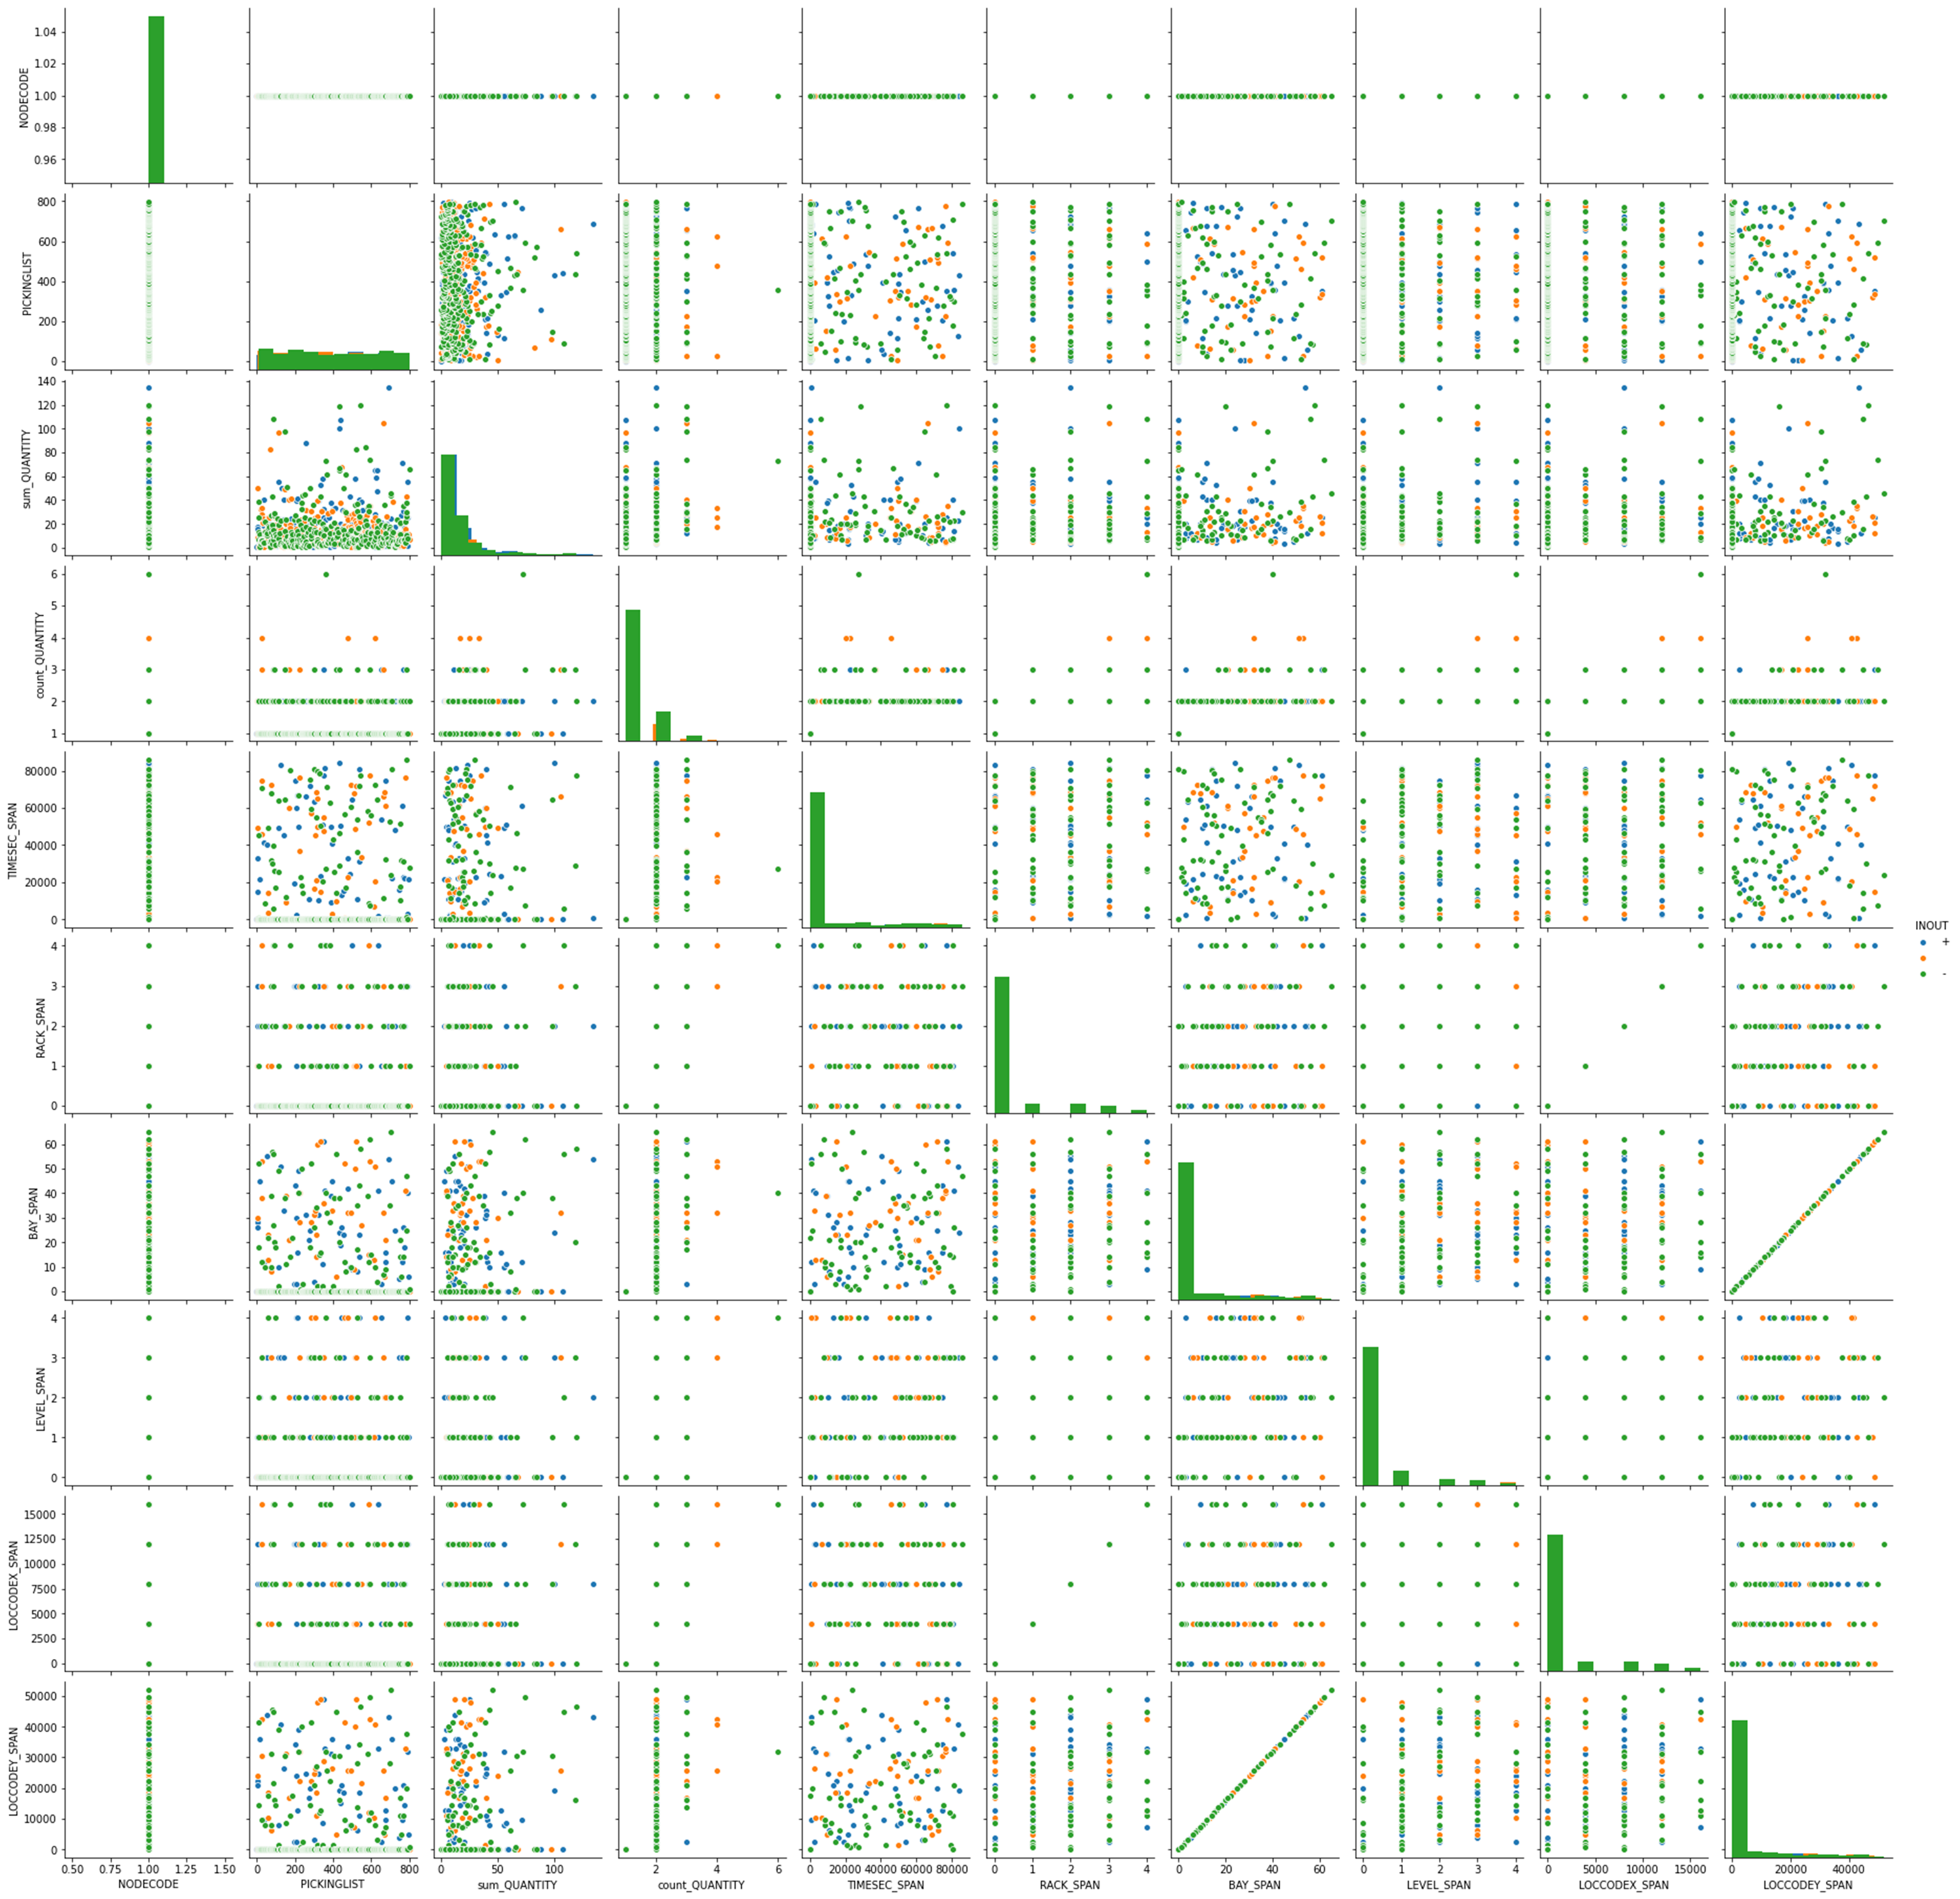
\includegraphics[width=1.0\textwidth]{SectionWarehouses/control_figures/fig_pick_pairplot.png}
\captionsetup{type=figure}
\caption{Pairplot of the key metrics to measure the picking lists.}
\label{fig_pick_pairplot}
\end{figure}

It is possible to evaluate the correlation between these metrics by using a correlation matrix. Figure \ref{fig_pick_corr} illustrates the correlation matrices of the inbound and outbound lists.\footnote{The source code of Figure \ref{fig_pick_corr} is available \href{https://github.com/aletuf93/logproj/blob/master/examples/WH_05\%20Warehouse\%20key\%20variables\%20exploration.ipynb}{here}.}

% INSERT fig_pick_corr
\begin{figure}[hbt!]
\centering
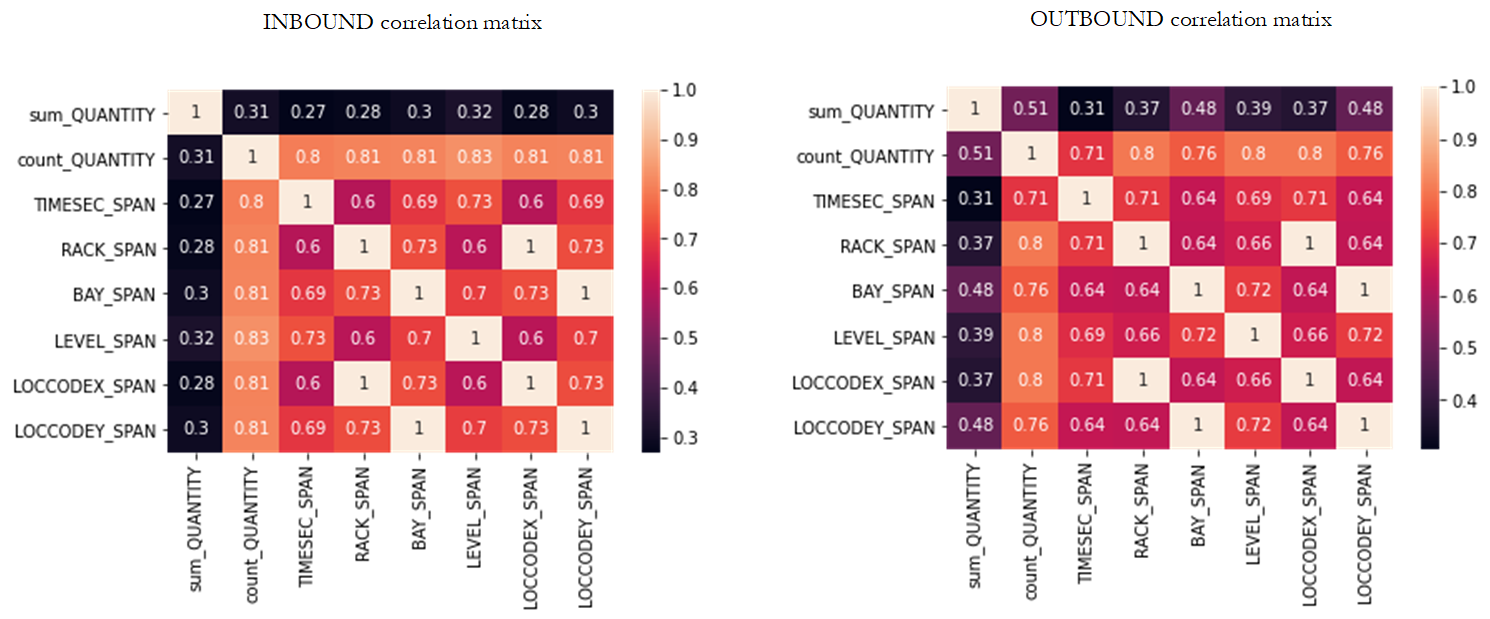
\includegraphics[width=1.0\textwidth]{SectionWarehouses/control_figures/fig_pick_corr.png}
\captionsetup{type=figure}
\caption{Inbound and outbound correlation matrices.}
\label{fig_pick_corr}
\end{figure}

\clearpage


\section{Vehicle routing (P10)}
Warehouse day-by-day involves the generation of the picking lists. This problem is equal to routing vehicle of a distribution system or assigning jobs to production machines. It is necessary to group picking activities such that the total travelled distance is minimised. It is a vehicle routing problem (VRP), where the nodes to visit are the storage locations ~\cite{Ratliff1983}.\par

Despite our introduction already defines a graph $G(V,A)$ with vertices and distances, sometime VRP within a storage system is more complex than it appears. First of all, the cost of picking is not only linked to the travelled distance. For a warehouse having thousands of SKUs, the cost of picking the wrong SKUs is much higher than travelling a few meters more. This is why random allocation and random picking policy are preferred when companies pay a high cost for a wrong picking (e.g. in the e-commerce).\par

Besides, VRP works offline, assuming that all the orders are known in advance. This is not always true for a WMS that can be frequently updated during the working shift. Finally, the set $V$ of the graph $G$ could have thousands of nodes (one for each storage location) resulting in a vast VRP problem, taking forever to solve.\par

Sometimes heuristics are used to approach this problem; e.g. by printing picking list for each zone of the warehouse when zoning is used. Warehouses with traversal directions use a single-direction snake path travelling through all the aisles of the warehouses for each picking list.\par

Generally, simulation is used to investigate the best picking list generation policy ~\cite{Chew1999, Hall1993, Kim2002, Petersen1999}. In truth, this work does not approach the problem since it is highly warehouse-dependent involving, in our opinion, too many parameters to be integrated into a single approach generalisable for any storage system.





%\clearpage
\bibliographystyle{ieeetr}
\bibliography{SectionWarehouses/control_ref}